\documentclass[a4paper,10pt]{article}
\usepackage{amssymb,amsmath}
\usepackage{graphicx}
\usepackage{html}
\usepackage[utf8x]{inputenc}
\usepackage{listings}

%opening
\title{\textit{lowmachSolver}: a low Mach number solver for spray simulation with OpenFOAM}
\author{Rodrigo B. Piccinini}

\begin{document}

\maketitle

\begin{abstract}
\textit{lowmachSolver} is an OpenFOAM solver that deals with two-phase flows composed of a continuous gaseous phase and a liquid dispersed phase.
\end{abstract}

\section{Introduction}
\textit{lowmachSolver} is an OpenFOAM solver that deals with two-phase flows composed of a continuous gaseous phase and a liquid dispersed phase. It is mainly based on \textit{dieselFOAM} and it was written only for purpose of my master thesis.

\subsection{OpenFOAM Code}

By \htmladdnormallink{OpenCFD own words}{http://www.openfoam.com/features/}:

\begin{quote}
The OpenFOAM  (Open Field Operation and Manipulation) CFD Toolbox is a free, open source CFD software package produced by OpenCFD Ltd. It has a large user base across most areas of engineering and science, from both commercial and academic organisations. OpenFOAM has an extensive range of features to solve anything from complex fluid flows involving chemical reactions, turbulence and heat transfer, to solid dynamics and electromagnetics. It includes tools for meshing, notably snappyHexMesh, a parallelised mesher for complex CAD geometries, and for pre- and post-processing. Almost everything (including meshing, and pre- and post-processing) runs in parallel as standard, enabling users to take full advantage of computer hardware at their disposal.

By being open, OpenFOAM offers users complete freedom to customise and extend its existing functionality, either by themselves or through support from OpenCFD. It follows a highly modular code design in which collections of functionality (e.g. numerical methods, meshing, physical models, …) are each compiled into their own shared library. Executable applications are then created that are simply linked to the library functionality. OpenFOAM includes over 80 solver applications that simulate specific problems in engineering mechanics and over 170 utility applications that perform pre- and post-processing tasks, e.g. meshing, data visualisation, etc. \end{quote} 

Details of OpenFOAM formulation are explained in \cite{jasak} and \cite{weller}.  From all the set of available solvers and libraries in OpenFOAM, the dieselFOAM solver and dieselSpray class (as implemented in version 1.7.1 of OpenCFD release) were the major pieces of code used in this work. To my knowledge, both were written by Niklas Nordin, \cite{nordin}.

The dieselSpray class handles the modeling of lagrangian particles and their submodels. Minor modifications were made in order to have more flexibility in boundary conditions and to adapt them to the experimental conditions.

The dieselFOAM solver couples the modeling of the lagrangian particles and the gas flow solution. The spray sources are explicitly treated and the coupling among variables is solved with PISO algorithm, see \cite{jasak} and \cite{ferziger}.

Minor modifications were added to the solution of low Mach number equations instead of the fully compressible formulation. They are briefly explained here, but the understanding requires from the reader some familiarity with OpenFOAM programming.

The thermodynamic pressure retained its original name \verb|p| and is the pressure used in the state equation:
\begin{verbatim}
<createFields.H>
volScalarField& p = thermo.p();                               
\end{verbatim} 
and in the lagrangian models:
\begin{verbatim}
<createSpray.H>
spray dieselSpray
(
    U,
    rho,
    p,
    T,
    composition,
    gasProperties,
    thermo,
    g
);\end{verbatim} 

A new scalar field was assigned to the dynamic pressure, \verb|volumeScalarField pd|:
\begin{verbatim}
<createFields.H>
 volScalarField pd
(
    IOobject
    (
        "pd",
        runTime.timeName(),
        mesh,
        IOobject::MUST_READ,
        IOobject::AUTO_WRITE
    ),
    mesh
);
\end{verbatim} 

The momentum equation was modified to be computed using the gradient of \verb|pd| instead of \verb|p| in the momentum predictor:
\begin{verbatim}
<UEqn.H>
     fvVectorMatrix UEqn
    (
        fvm::ddt(rho, U)
      + fvm::div(phi, U)
      + turbulence->divDevRhoReff(U)
     ==
        rho*g
      + dieselSpray.momentumSource()
    );

    if (momentumPredictor)
    {
        solve(UEqn == -fvc::grad(pd));
    }
\end{verbatim} 

Finally, the the pressure equation is now a Poisson equation for the dynamic pressure and it uses the thermodynamic pressure for computing the density.
\begin{verbatim}
<pEqn.H>

  fvScalarMatrix pdEqn
  (
      fvc::ddt(psi,p)
      + fvc::div(phi)
      - fvm::laplacian(rho*rUA, pd)
      ==
      Sevap
  );
\end{verbatim} 
where \verb|psi| or $\Psi$ is the isothermal compressibility. For an ideal gas:
\begin{equation}
 \rho=p\Psi=\frac{p}{RWT} \, .
\end{equation}

The time-dependence of the thermodynamic pressure was neglected (valid for open domains) and the therm \verb|fvc::ddt(psi,p)| vanishes.


\section{Folder Structure}

The thesis work is organized in a typical SVN folder structure: 
\begin{verbatim}
--- branches
--- tags
--- trunk
--- wiki
\end{verbatim}
After finishing the thesis, everything was merged to \textbf{trunk} folder and the others were left empty.

\htmladdnormallink{./trunk}{../../} folder has the following structure:
\begin{verbatim}
--- trunk
    +-- case
    |   +-- halle			test case from Sommerfeld, and H.-H. Qiu (not fully finished).
    |   |   +-- 2D				2D mesh and case setup.
    |   |   +-- exp				experimental data.
    |   |   +-- misc			miscellaneous Python scripts.
    |   |
    |   +-- sydney			test case from Chen et al (Sydney University). In the thesis.
    |       +-- case			fine mesh setup.
    |       +-- case.coarse			coarse mesh setup.
    |       +-- ic.coarse			Initial conditions for the coarse mesh case.
    |       +-- ic.fine			Initial conditions for the fine mesh case.
    |       +-- misc			miscellaneous Python scripts for plotting results and building mesh.
    |
    +-- code
    |   +-- 1.7.x			code based on 1.7.1 release from OpenCFD
    |       +-- lowmachLib			lagrangian spray lib.
    |       +-- lowmachSolver		low Mach number solver coupled with lowmachLib.
    |       +-- myLiquids			acetone liquid and vapor properties
    |       +-- mypdfs			spray probability density functions
    |
    +-- paper			thesis results in paper format
    |   +-- elsevier			Elsevier latex class
    |
    +-- ppt				presentation given in 2011/nov/25 at ITA.
    |   +-- imgs				figures in presentation.
    |       +-- visit				figures post-processed in visIT
    |
    +-- thesis			thesis .tex source files.
    |   +-- figuras			figures with .dat files for each of the subsequent thesis appendix and chapters.
    |       +-- appA1
    |       +-- appA2
    |       +-- appA3
    |       +-- chap1
    |       +-- chap2
    |       +-- chap3
    |       +-- chap4
    |       +-- chap5
    |
    +-- tutorial			this tutorial source files.
	+-- html				html files from latex2html.
\end{verbatim}


\section{Compiling}

Compiling was tested with Ubuntu Natty (numbered 11.04) and .deb package of OpenFOAM 1.7.1 released by OpenCFD.


\htmladdnormallink{http://www.openfoam.org/archive/1.7.1/download/}{http://www.openfoam.org/archive/1.7.1/download/}


Development tools for Ubuntu must be present. They can be installed by:
\begin{verbatim}
 sudo apt-get install build-essential flex bison cmake zlib1g-dev qt4-dev-tools libqt4-dev gnuplot libreadline-dev libxt-dev
\end{verbatim}
For parallel runs, installation of the following libraries is also required:
\begin{verbatim}
sudo apt-get install libscotch-dev libopenmpi-dev
\end{verbatim}

Code is located in \htmladdnormallink{./trunk/code/1.7.x/}{../../code/1.7.x}
\begin{verbatim}
--- trunk
    +-- code
        +-- 1.7.x			code based on 1.7.1 release from OpenCFD
            +-- lowmachLib			lagrangian spray lib.
            +-- lowmachSolver			low Mach number solver coupled with lowmachLib.
            +-- myLiquids			acetone liquid and vapor properties
            +-- mypdfs				spray probability density functions
\end{verbatim}

Inside \htmladdnormallink{./trunk/code/1.7.x/}{../../code/1.7.x}, the following scripts may be issued to:
 \begin{verbatim}
# ./Allwmake			compile the solver and all needed libraries.
# ./CleanSrc			clean the source files for a new compiling.
# ./CleanAll			clean both source and binary files for a new compiling.
\end{verbatim}

\textbf{Allwmake} script will make a user installation after compiling the code.

\section{Running}
lowmachSolver can be run as any OpenFOAM solver with usual options:
\begin{verbatim}
#lowmachSolver -help

Usage: lowmachSolver [-parallel] [-case dir]  [-help]
\end{verbatim}

See Test Case section \ref{sydney} for an example.

\section{Test Case}\label{sydney}

This is the test case used to provide results for the thesis. It consists of the numerical simulation of the experiment performed by \cite{chen} in Sydney University.

\htmladdnormallink{http://dx.doi.org/10.1016/j.ijmultiphaseflow.2005.09.002}{http://dx.doi.org/10.1016/j.ijmultiphaseflow.2005.09.002}

Case folder structure
\begin{verbatim}
--- case
    +-- 0			initial and boundary conditions
    +-- chemkin			chemkin files
    +-- constant		mesh and physical properties
    +-- system			solution parameters
\end{verbatim}

\paragraph{./case/0/}
Folder \textbf{case/0/} contains initial and boundary conditions. The type of each boundary conditions is presented in the thesis \cite{piccinini_msc} and may be directly read in the files as well.

Iinitial conditions of the gaseous flow were obtained by simulating only the gas flow in \htmladdnormallink{../cases/sydney/ic.fine/}{../cases/sydney/ic.fine/} and \htmladdnormallink{../cases/sydney/ic.coarse/}{../cases/sydney/ic.coarse/}.

\paragraph{./case/chemkin/}
Chemkin folder contains chemical kinetic and thermodynamic data of all present species in gas phase. No chemical reaction is present. Thermodynamic and transport properties of acetone in liquid phase are computed "inside" the code.

\paragraph{./case/constant/}
\begin{description}
 \item[turbulenceProperties] informs that the simulation is turbulent and it is using RANS modeling.

 \item[RASProperties] selects the turbulence model: standard k-epsilon.

 \item[g] defines the gravity vector field.

 \item[thermophysicalProperties] defines the thermodynamic and transport models for gas and liquid phases.
\begin{verbatim}
thermoType      hsPsiMixtureThermo<reactingMixture<gasThermoPhysics>>; 
\end{verbatim}

hsPsiMixtureThermo computes enthalpy for combustion mixture based on sensible enthalpy $h_s$ and compressibility $\Psi$.
reactingMixture  is a combustion mixture using thermodynamics and reaction schemes.
gasThermoPhysics is a type definition for \verb|sutherlandTransport<specieThermo<janafThermo<perfectGas>>>|. 

 \item[combustionProperties] no combustion is present, so the important information is \verb|ignite off;|.

 \item[chemistryProperties] chemical reactions are not solved. Just like before, \verb|chemistry off;| is what matters.
 
 \item[injectorProperties] defines almost all droplet properties in the injector exit: position, temperature, velocity magnitude and direction, mass flow rate and parcels per second (nParcels). Droplet diameter is specified in next file.

 \item[sprayProperties] defines all droplet modeling and the diameter probability density function (pdf).

The time step for integrating droplet equations is the minimum between momentum and heat transfer characteristic times divided by \verb|subCycles|. \verb|dtInjection| was added to limit the number of parcels in the domain: only one parcel is added during the specified time interval.
\begin{verbatim}
subCycles          2;
dtInjection		1e-9;           		     
\end{verbatim} 

Atomization is modeled statistically by the pdf function and no physical modeling is used.
\begin{verbatim}
atomizationModel        off;\end{verbatim} 

Since acetone is a highly volatile fuel, droplets are more likely to evaporate before undergo secondary break-up instabilities.
\begin{verbatim*}
includeOscillation      off;
//breakupModel    TAB;
//breakupModel    ETAB;
//breakupModel    ReitzDiwakar;
breakupModel    off;\end{verbatim*}

The injector type is set.
\begin{verbatim}
injectorModel           hollowConeInjector;\end{verbatim} 

Collision model is not used since the spray is dilute.  Evaporation, heat transfer, drag and droplet dispersion is modeled as discussed in \cite{piccinini_msc}.
\begin{verbatim}
collisionModel  off;
evaporationModel standardEvaporationModel;
heatTransferModel RanzMarshall;
dispersionModel stochasticDispersionRAS;
dragModel       standardDragModel;\end{verbatim} 

Added the lognormal pdf to the available pdfs. It is used to sample droplet diameter for injection.
\begin{verbatim}
hollowConeInjectorCoeffs
{
    dropletPDF
    {
			pdfType         lognormal;
    }
}   
\end{verbatim} 

 \end{description}

\subsection{Solver Output}

Basic information about the spray and execution timing followed by extremal values of temperature, density and dynamic pressure.
\begin{verbatim}
Number of parcels in system.... | 29921
Injected liquid mass........... | 6.05092 mg
Liquid Mass in system.......... | 0.522468 mg
SMD, Dmax...................... | 16.0027 mu, 42.7612 mu
ExecutionTime = 102.28 s  ClockTime = 104 s
T max/min : 298 275.949
rho max/min : 1.28461 1.1644
pd max/min : 100000 99966.9
\end{verbatim}

Mass flow rates trough defined patches (walls are being called as such, but they are actually the far boundary).
\begin{verbatim}
Courant Number mean: 0.00232359 max: 0.242796
MassFlows:   nozzle = -3.43682e-05  coflow = -0.000852618  outlet = 0.00100765  walls = -0.00012141
Time = 0.330113
\end{verbatim}

The following lines show the sequence equations are solved: first spray is updated, then all transport equations are solved. "\verb|Solving for rho|" presents zero residual and iterations because it is being explicitly solved.
\begin{verbatim}
Evolving Spray
Solving chemistry
diagonal:  Solving for rho, Initial residual = 0, Final residual = 0, No Iterations 0
DILUPBiCG:  Solving for Ux, Initial residual = 5.77748e-07, Final residual = 5.2592e-09, No Iterations 1
DILUPBiCG:  Solving for Uy, Initial residual = 2.6999e-05, Final residual = 7.62742e-11, No Iterations 2
DILUPBiCG:  Solving for Uz, Initial residual = 5.88654e-05, Final residual = 7.16722e-08, No Iterations 1
DILUPBiCG:  Solving for aC3H6O, Initial residual = 3.79856e-07, Final residual = 8.03328e-10, No Iterations 1
DILUPBiCG:  Solving for O2, Initial residual = 3.88094e-07, Final residual = 3.96676e-10, No Iterations 1
DILUPBiCG:  Solving for CO2, Initial residual = 0, Final residual = 0, No Iterations 0
DILUPBiCG:  Solving for H2O, Initial residual = 0, Final residual = 0, No Iterations 0
DILUPBiCG:  Solving for hs, Initial residual = 5.01197e-07, Final residual = 1.08758e-09, No Iterations 1
\end{verbatim}

The following step is the PISO loop, which might be repeated more than once (I used 3 to 5 loops).
\begin{verbatim}
DICPCG:  Solving for pd, Initial residual = 0.0447168, Final residual = 9.75726e-10, No Iterations 185
diagonal:  Solving for rho, Initial residual = 0, Final residual = 0, No Iterations 0
time step continuity errors : sum local = 3.66451e-16, global = -2.59971e-18, cumulative = -7.82325e-16
\end{verbatim}

For last, solution of k-epsilon equations.
\begin{verbatim}
DILUPBiCG:  Solving for epsilon, Initial residual = 5.26145e-07, Final residual = 5.43398e-10, No Iterations 1
DILUPBiCG:  Solving for k, Initial residual = 1.22238e-07, Final residual = 1.64783e-10, No Iterations 1
\end{verbatim}



\subsection{Some Results}

\begin{figure}
 \centering
 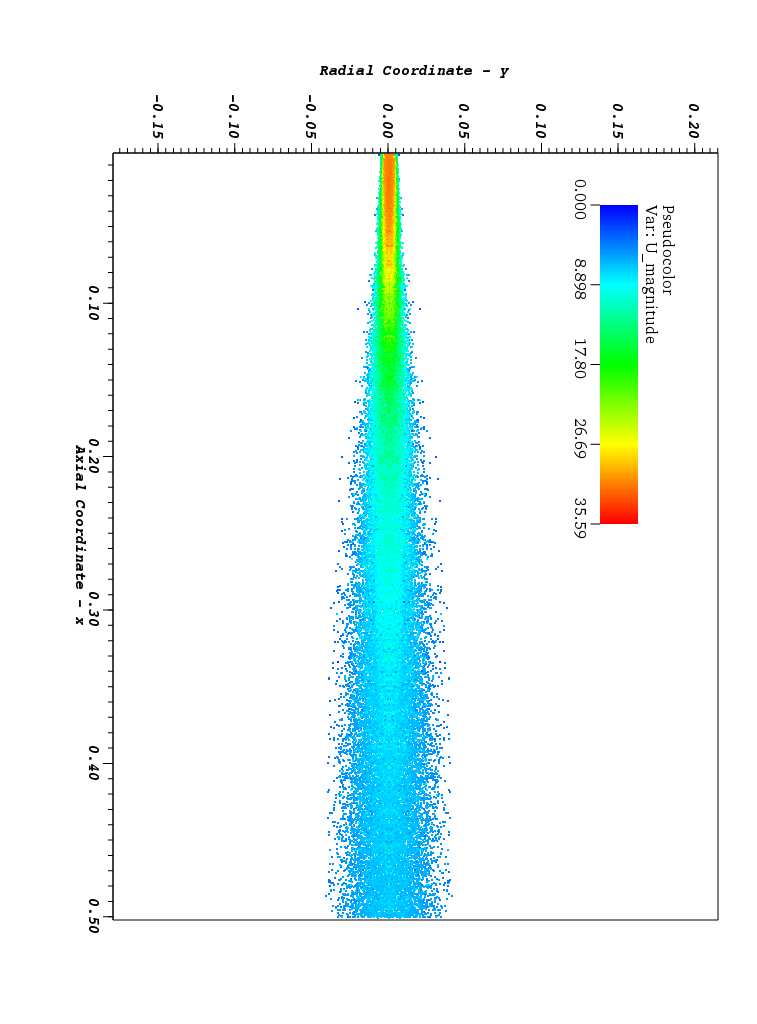
\includegraphics[angle=90,width=\textwidth]{../thesis/figuras/appA2/visit_U.png}
 \caption{Magnitude of droplet velocities. The computational domain is only half of the shown above, it is here mirrored for visualization purpose.}
 \label{fig: dropU}
\end{figure}

\begin{figure}
\begin{center}
 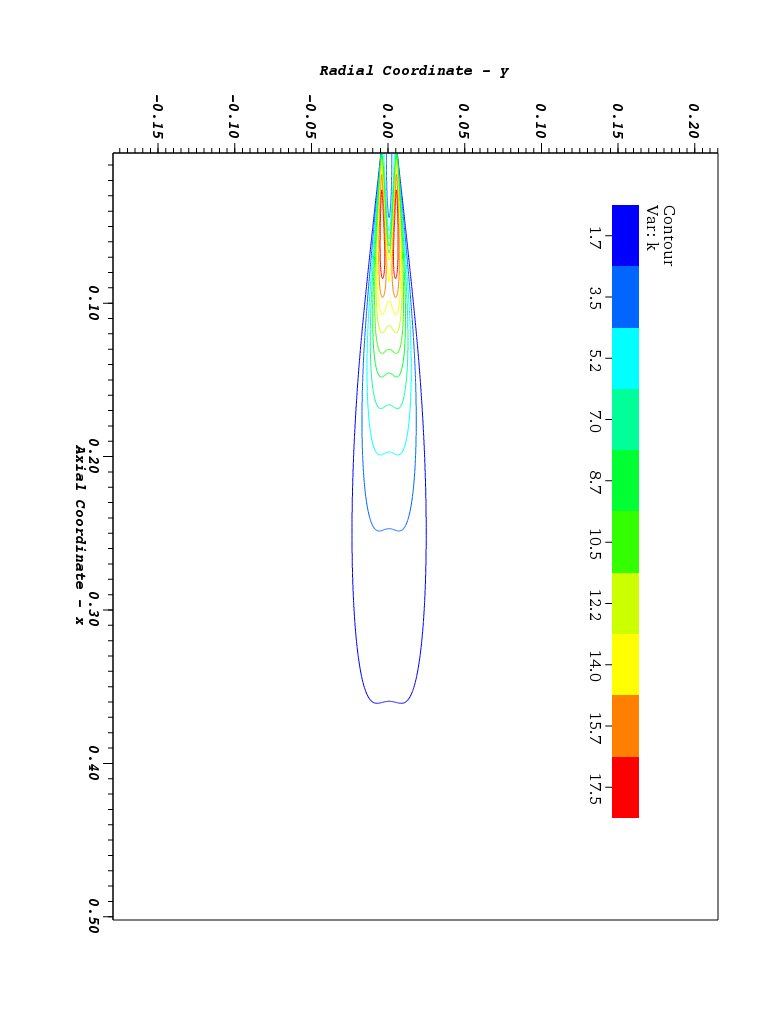
\includegraphics[angle=90,width=\textwidth]{../thesis/figuras/appA2/visit_k.png}
 \end{center}
 \caption{Gas mean turbulent kinetic energy. The computational domain is only half of the shown above, it is here mirrored for visualization purpose.}
 \label{fig: field_k}
\end{figure}


\section{Links}

Openfoam:
\htmladdnormallink{OpenFOAM}{http://www.openfoam.com/}
\htmladdnormallink{OpenFOAM-extend}{http://www.extend-project.de}

Academics:
\htmladdnormallink{ITA}{http://www.ita.br}
\htmladdnormallink{LCFT/ITA}{http://lcft.mec.ita.br}


\bibliographystyle{plain}
\bibliography{../thesis/references}
\end{document}
